% Exemplo de relatório técnico do IC

% Criado por P.J.de Rezende antes do Alvorecer da História.
% Modificado em 97-06-15 e 01-02-26 por J.Stolfi.
% modificado em 2003-06-07 21:12:18 por stolfi
% modificado em 2008-10-01 por cll
% modificado em 2010-03-16 17:56:58 por stolfi
% modificado em 2012-09-25 para ajustar o pacote UTF8. Contribuicao de Rogerio Cardoso
% \def\lastedit{2015-03-18 00:52:20 by bit}

\nonstopmode % PARA RODAR LATEX EM BATCH MODE
\documentclass[11pt,twoside]{article}

\usepackage{techrep-ic}
\usepackage{amsmath}
\usepackage{amssymb}
\usepackage{subcaption}
\usepackage[english]{babel}
\usepackage[utf8]{inputenc}
\usepackage[margin=1in]{geometry}
\usepackage[
  style=numeric,
  sorting=none
]{biblatex}
\addbibresource{references.bib}
\usepackage{xcolor}
\usepackage[hidelinks]{hyperref}
\usepackage[noabbrev, capitalise]{cleveref}
\usepackage[cache=false]{minted}
\usemintedstyle{borland}

\begin{document}

%%% PÁGINA DE CAPA %%%%%%%%%%%%%%%%%%%%%%%%%%%%%%%%%%%%%%%%%%%%%%%
% 
% Número do relatório
\TRNumber{41} % Dois dígitos
\TRYear{23} % Dois dígitos
\TRMonth{12} % Numérico, 01-12
\TRAuthor{Paulo Pacitti \and Julio López}
\TRTitle{Lightweight Cryptography with Ascon in \texttt{riscv64}}
\TRMakeCover

%%%%%%%%%%%%%%%%%%%%%%%%%%%%%%%%%%%%%%%%%%%%%%%%%%%%%%%%%%%%%%%%%%%%%%
% O que segue é apenas uma sugestão - sinta-se à vontade para
% usar seu formato predileto, desde que as margens tenham pelo
% menos 25mm nos quatro lados, e o tamanho do fonte seja pelo menos
% 11pt. Certifique-se também de que o título e lista de autores
% estão reproduzidos na íntegra na página 1, a primeira depois da
% página de capa.
%%%%%%%%%%%%%%%%%%%%%%%%%%%%%%%%%%%%%%%%%%%%%%%%%%%%%%%%%%%%%%%%%%%%%%

%%%%%%%%%%%%%%%%%%%%%%%%%%%%%%%%%%%%%%%%%%%%%%%%%%%%%%%%%%%%%%%%%%%%%%
% Nomes de autores ABREVIADOS e titulo ABREVIADO,
% para cabeçalhos em cada página.
%
\markboth{Pacitti, López}{Lightweight Cryptography with Ascon in riscv64}
\pagestyle{myheadings}
\thispagestyle{empty}

%%%%%%%%%%%%%%%%%%%%%%%%%%%%%%%%%%%%%%%%%%%%%%%%%%%%%%%%%%%%%%%%%%%%%%
% TÍTULO e NOMES DOS AUTORES, completos, para a página 1.
% Use "\\" para quebrar linhas, "\and" para separar autores.
%
\title{Lightweight Cryptography with Ascon in riscv64}

\author{Paulo Pacitti\thanks{Institute of Computing, UNICAMP. \texttt{p185447@dac.unicamp.br}} \and
  Julio  López\thanks{Associate Professor, Institute of Computing, UNICAMP. \texttt{jlopez@ic.unicamp.br}}}
\date{}
\maketitle

%%%%%%%%%%%%%%%%%%%%%%%%%%%%%%%%%%%%%%%%%%%%%%%%%%%%%%%%%%%%%%%%%%%%%%

\begin{abstract}
  Sed quis lorem magna. Sed sit amet ullamcorper massa, sit amet placerat lectus. Suspendisse pulvinar ipsum sed enim commodo, ac malesuada lectus finibus. Aliquam eu eros eleifend, interdum nisi faucibus, viverra sapien. Vivamus lobortis a lectus eu rutrum.
  Quisque in est sit amet libero sollicitudin ornare a sed ipsum. Suspendisse potenti.
  Aliquam sit amet nisi sed nulla tincidunt imperdiet. Pellentesque elementum lacus eget
  dolor gravida lobortis. Sed placerat lacinia nisi, sed varius turpis facilisis ac.
\end{abstract}

\section{Introduction}
Inspired by the works of the UNICAMP's Laboratory of Security and Cryptography in the optimization of cryptographic algorithms for the ARM architecture \cite{Fujii2017a}, the NIST Lightweight Cryptography competition winner algorithm \cite{turan2023status}, and the RISC-V open architecture, this research aims to explore the Ascon family of algorithms \cite{asconv12nist} on the RISC-V 64-bit architecture and wether it's possible to optmize it for this architecture. There are other works that have explored the Ascon family of algorithms \cite{jellema2019optimizing} that explores the Ascon algorithm in RISC-V, but in the 32-bit version and benchmarking in a FPGA chip. It was used in this paper for benchmarking a 64-bit RISC-V chip, the Allwinner D1.

The approach was to analyze the Ascon algorithm design and 3 different implementations. All the implementations tested are written in C. The first implementation \texttt{ref} is the reference implementation of Ascon, written by Ascon team \cite{asconc2023}. The second one is \texttt{opt64}, and optmized implementation for a generic 64-bit architecture system, also developed by the Ascon team. The  third implementation was the main objective of this research, named \texttt{ascon-v} \cite{asconv2023}, this implementation is focused on producing a optmized version for the RISC-V 64-bit architecture. The research was focused on trying to improve the basic blocks of the Ascon family of algorithms. Because of that, the analysis, optimizations and results are focused on the \textsc{Ascon-128}, which is the \textit{de facto} AEAD standard of the Ascon family.

\section{Ascon}

Ascon is a family of algorithms for lighweight cryptography, designed to be used in constrained environments,
like embedding computing. Designed by cryptographers from Graz University of Technology, Infineon Technologies, Intel Labs, and Radboud University, Ascon has been selected as the new standard for lightweight cryptography in the 2019–2023 NIST Lightweight Cryptography competition. The Ascon family is mainly composed by 4 algorithms: \textsc{Ascon-128}, \textsc{Ascon-128a}, \textsc{Ascon-Hash} and \textsc{Ascon-Hasha}. There's also variants \textsc{Ascon-80pq}, \textsc{Ascon-Xof}, \textsc{Ascon-Xofa}, where the first it's a version of AEAD with an increased key size of 160 bits and the latter two are versions of the hash algorithm but they produce hash outputs of arbitrary
length, just changing the number of rounds necessary for it. The \cref{table:1} shows the parameters of the recommended AEAD schemes from the Ascon family of algorithms, where this article will focus on the \textsc{Ascon-128}. The algorithms use the encryption function $\textit{E}_{k,r,a,b}$ and the decryption function $\textit{D}_{k,r,a,b}$ where $k$ is the key size, $r$ is the rate (data block) size, $a$ is the tag size, $b$ is the data block size, and $p^a$ and $p^b$ are the number of rounds used in the many permutations used across the algorithms. The encryption $\textit{E}_{k,r,a,b}(K, A, N, P) = (C, T)$ receives a key $K$, an associated data $A$, a nonce $N$ and a plaintext $P$ and returns a ciphertext $C$ and a tag $T$. The decryption $\textit{D}_{k,r,a,b}(K, A, N, C, T) \in \{P, \perp\}$ receives a key $K$, an associated data $A$, a nonce $N$, a ciphertext $C$ and a tag $T$ and returns the plaintext $P$ if the verification of the tag is correct, otherwise it returns the $\perp$ error.


\begin{table}
  \centering
  \begin{tabular}{|c|c|cccc|cc|}
    \hline
    \textbf{Name}       & \textbf{Algorithms}                     & \textbf{key} & \textbf{nonce} & \textbf{tag} & \textbf{data block} & \textbf{$p^a$} & \textbf{$p^b$} \\ \hline
    \textsc{Ascon-128}  & \textit{E}, $\textit{D}_{128,64,12,6}$  & 128          & 128            & 128          & 64                  & 12             & 6              \\ \hline
    \textsc{Ascon-128}a & \textit{E}, $\textit{D}_{128,128,12,8}$ & 128          & 128            & 128          & 128                 & 12             & 8              \\ \hline
  \end{tabular}
  \caption{Ascon AEAD parameters}
  \label{table:1}
\end{table}

Ascon lightweight properties comes from using the simple bitwise operations that majority of microcontrollers have, like XOR, AND, OR, NOT, and bitwise rotations. The algorithm is based on a sponge construction, which is a cryptographic primitive that can be used to build cryptographic hash functions, pseudorandom functions, and authenticated encryption schemes, like the SHA-3 (also know as "Keccak") \cite{bertoni2015keccak} algorithm. The sponge construct consists in keeping a finite internal state that takes input streams (absorb) to update the state and output streams (squeeze) to produce the output from the internal state, as it's displayed in \cref{fig:1}.

\begin{figure}[h]
  \centering
  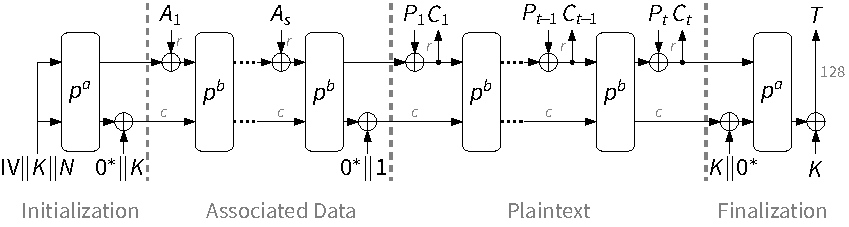
\includegraphics[scale=0.8]{assets/aead_encrypt.pdf}
  \caption{Ascon permutation S-box.}
  \label{fig:1}
\end{figure}

The Ascon state is composed by 5 64-bit words, also named as Ascon words, resulting in a 320-bit internal state. This internal state is then manipulated using the Ascon permutation procedure.

\subsection{Permutation}

The Ascon permutation is the main building block of the Ascon family of algorithms and consists in 3 stages: round constant addition, a substitution-layer (S-Box) and a linear diffusion layer. It's then used in the AEAD encryption and decryption procedures in the form of $p^a$ and $p^b$, where $p$ is the permutation and $a$ and $b$ are the number of rounds. The parameters $a$ and $b$ is different for each algorithm of the Ascon family, but the permutation is the same for all of them, as it's displayed in \cref{table:1}.

As the Ascon state has 5 64-bit words, the round constant addition consists in XORing the round constant with the second Ascon word. The round constant is a 64-bit value that is different for each round. \color{orange} (add round constants table?) \color{black} The substitution-layer consists in applying a S-Box to the Ascon state. The S-Box is a 5x5 matrix of 64-bit words, where each word is a 5-bit S-Box. The S-Box is applied to each Ascon word, resulting in a new Ascon state as displayed in \cref{fig:2a}. The linear diffusion layer consists in the linear diffusion function $x_i \leftarrow \Sigma_i(x_i)$ applied to each Ascon word $x_i$, where each word has a specific function definition $\Sigma_i(x_i)$. The linear diffusion function definitions are shown in \cref{fig:2b}.

\begin{figure}
  \centering
  \begin{subfigure}[b]{0.4\textwidth}
    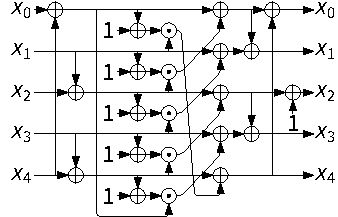
\includegraphics[scale=1]{assets/sbox.pdf} \\
    \caption{Ascon permutation S-box.}
    \label{fig:2a}
  \end{subfigure}
  \hspace*{0.01\textwidth}
  \begin{subfigure}[B]{0.55\textwidth}
    \begin{align*}
       & x_0 \leftarrow \Sigma_{0}(x_0) = x_0 \oplus (x_0 \ggg 19) \oplus (x_0 \ggg 28)          \\
       & x_1 \leftarrow \Sigma_{1}(x_1) = x_0 \oplus (x_1 \ggg 61) \oplus (x_0 \ggg 39)          \\
       & x_2 \leftarrow \Sigma_{2}(x_2) = x_2 \oplus (x_2 \ggg \ \, 1) \oplus (x_2 \ggg \ \,  6) \\
       & x_3 \leftarrow \Sigma_{3}(x_3) = x_3 \oplus (x_3 \ggg 10) \oplus (x_3 \ggg 17)          \\
       & x_4 \leftarrow \Sigma_{4}(x_4) = x_4 \oplus (x_4 \ggg \ \,  7) \oplus (x_4 \ggg 41)
    \end{align*}
    \vspace*{0.07\textwidth}
    \caption{Ascon linear diffusion layer}
    \label{fig:2b}
  \end{subfigure}
  \caption{S-box and linear diffusion layers in the Ascon permutation.}
  \label{fig:2}
\end{figure}

\begin{listing}[ht!]
  \begin{minted}{c}
    // Ascon state with 5 64-bit words.
    typedef struct {
        uint64_t x[5];
    } ascon_state_t;

    // Bitwise rotation to the right.
    static inline uint64_t ROR(uint64_t x, int n) {
        return x >> n | x << (-n & 63);
    }

    // Ascon permutation round function.
    static inline void ROUND(ascon_state_t *s, const uint8_t C) {
        ascon_state_t t;
        /* round constant layer */
        s->x[2] ^= C;
        /* substitution layer */
        s->x[0] ^= s->x[4];
        s->x[4] ^= s->x[3];
        s->x[2] ^= s->x[1];
        t.x[0] = s->x[0] ^ (~s->x[1] & s->x[2]);
        t.x[1] = s->x[1] ^ (~s->x[2] & s->x[3]);
        t.x[2] = s->x[2] ^ (~s->x[3] & s->x[4]);
        t.x[3] = s->x[3] ^ (~s->x[4] & s->x[0]);
        t.x[4] = s->x[4] ^ (~s->x[0] & s->x[1]);
        t.x[1] ^= t.x[0];
        t.x[0] ^= t.x[4];
        t.x[3] ^= t.x[2];
        t.x[2] = ~t.x[2];
        /* linear diffusion layer */
        s->x[0] = t.x[0] ^ ROR(t.x[0], 19) ^ ROR(t.x[0], 28);
        s->x[1] = t.x[1] ^ ROR(t.x[1], 61) ^ ROR(t.x[1], 39);
        s->x[2] = t.x[2] ^ ROR(t.x[2], 1) ^ ROR(t.x[2], 6);
        s->x[3] = t.x[3] ^ ROR(t.x[3], 10) ^ ROR(t.x[3], 17);
        s->x[4] = t.x[4] ^ ROR(t.x[4], 7) ^ ROR(t.x[4], 41);
    }
  \end{minted}
  \caption{Ascon permutation used in \texttt{ref} implementation.}
  \label{lst:1}
\end{listing}

\subsection{Encryption}

\subsection{Decryption}

\section{RISC-V}

\section{Implementation}

The device used for this research is the MangoPi MQ-Pro, a SBC powered with a Allwinner D1 chip and 1GB DDR3 of RAM, with Wi-Fi, Bluetooth and HDMI video output. The Allwinner D1 chip contains a T-Head Xuantie C906 core, a RISC-V 64-bit 1GHz CPU supporting RV64GC ISA. The board runs Ubuntu Server 23.04, running the 6.2.0-36-generic version of the Linux kernel. For compiling the implementation in C, it was used the RISC-V GNU Compiler Collection (GCC) version 12.2.0 \cite{riscvgnutoolchainv2023} through cross-compilation with Newlib, using a MacBook Pro with an Apple M1 chip. The implementation techniques that are going to be described next were used in the \texttt{ascon-v} implementation to attempt to overcome the performance of \texttt{ref} and \texttt{opt64} implementations.

Since it's a 64-bit architecture, it's possible to store each of the 5 64-bit Ascon word in one register at a time. The use of the library \texttt{<stdint>} becomes very useful since it's possible to define exactly the bistring size representation, not being dependent on what the C types \texttt{long long} and \
\texttt{unsigned long long} translates to. The Ascon permutation S-box translates to what it can be seen in the \cref{lst:1}, as well the round constant addition and linear diffusion stages.

Ascon words, used to mantain the state in the sponge construct, are big endian. The reference implementation merges data to these words by loading and storing bytes using big-endianess, requiring operations to fill the right-side with zeros. However, RISC-V, as like most of other ISAs, is little endian, making bitwise operations slower than it could be if the architecture had the same endianess than the algorithm. It's possible to implement an opmitization considering this issue by handling the data as little-endian in the implementation and reversing the endianess when merging data to the Ascon words \cite{jellema2019optimizing}. This turns out to be way more effective than operating in data in big endinaness since loading bytes and other biwise operations does not need to fill the right-side of the bistring with zeros, as it is in big-endinaness. That way, the cost of reversing the endianess of little-endian 64-bit bistring is lower than the cost of loading data in big-endianess.

Another minor improvement is done in the finalization of the ciphertext procedure that happens in the decryption procedure. After retrieving the last section of the decryption of the ciphertext into plaintext, the algorithm defined that the Ascon state needs to XORed with the bitwise string consisting in the last piece of plaintext, the value of 1, and padded bitwise 0 bitstring of zeros until it reachs the 320-bit size of the Ascon state. \cref{eq:2} displays the operation, where $S_r$ is the Ascon state, $\tilde{P_t}$ is the last piece of plaintext, $\tilde{C_t}$ is the last piece of ciphertext, and $0^*$ is the bitstring of zeros until it reachs the 320-bit size of the Ascon state:

\begin{align}
   & \tilde{P_{t}} \leftarrow  {\left \lfloor S_{r}  \right \rfloor}_{\left| \tilde{C_{t}} \right|} \oplus \tilde{C_{t}} \label{eq:2} \\
   & S_r \leftarrow S_r \oplus (\tilde{P_{t}} || 1 || 0^{*}) \label{eq:3}
\end{align}

The \texttt{ref} and \texttt{opt64} implementations do this operation by cleaning the first (in big-endianess representation) $| \tilde{C_{t}} |$ bytes of $S_r$, then ORing with $\tilde{C_t}$ to load these bytes into $S_r$. Since $S_r \oplus \tilde{P_t} = S_r \oplus  (S_r \oplus \tilde{C_t}) = 0 \oplus \tilde{C_t} = \tilde{C_t}$, $S_r \oplus \tilde{P_t}$ is equivalent to $S_{r} \ |= \tilde{C_t}$, after the first $| \tilde{C_{t}} |$ bytes of $S_r$ are cleared. In \texttt{asconv}, in the purpose of trying to improve the performance, the operations done in \cref{eq:2} and \cref{eq:3} are done with biwise shift instructions, as it's displayed in \cref{eq:4} and \cref{eq:5}:

\begin{align}
   & r \leftarrow (S_r \oplus \tilde{C_{t}}) \ggg (320 - | \tilde{C_{t}}|) \lll (320 - | \tilde{C_{t}} |) \ | \ (1|0^*) \label{eq:4} \\
   & S_r \leftarrow S_r \oplus r \label{eq:5}
\end{align}

It was used optimization techiniques to improve the performance of the implementation by using compile-time optimizations. Because many of the operations used in the Ascon are used very often, it's faster to implement then as \texttt{inline} functions, so the compiler can optimize the code by inlining the function calls. The \texttt{ROUND} function, used in the Ascon permutation, is a good example of this, as it's used in every round of the permutation. The permutations $p^6$ and $p^{12}$, used in \textsc{Ascon128}, instead of retrieving the value of their round constants in runtime, it's better to implement as inline functions to eliminate the time of getting the specific round constant value for that round. Compilation flags were also used to improve the performance, using \texttt{-O2} optimization, \texttt{-march=rv64gc} to enable the RV64GC ISA, and \texttt{-mtune=thead-c906} to enable the compiler to optimize the code for the C906 CPU core inside the Allwinner D1 chip.

\section{Results}

Considering $t$ the elapsed time to run encryption/decryption of a plaintext/ciphertext, the resolution $R$ of the timer used to measure the time of the C906 core to be 45 nanoseconds  \cite{10179399}, $F$ the CPU frequency, the number of clock cycles used in encryption/decryption can be calculated \cref{eq:1}:

\begin{equation}
  C = t \times R \times F \times \frac{10^{9}}{60} \label{eq:1}
\end{equation}

\section{Future}

The Ascon permutation proposed in the specification, shown in \cref{lst:1}, also allows the use of parallelism that could accelerate the performance. Unfortunately, the Allwiner D1 chip does not support vectorial instructions and is single-core only, so the analysis of the use of the vectorial extensions will be left for future work.

As we can see, the RV64GC instructions do not allow great optimizations from the architecture itself since it doesn't have any special instructions to accelerate operations of the Ascon128. However, RISC-V does have instructions extensions in development, and even ratfied, that could improve the performance of Ascon. Such cryptographic specialized instruction extenstions are divided in scalar and vectorial.

The Scalar Cryptography set of extensions (Zbkb, Zbkc, Zbkx, Zknd, Zkne, Zknh, Zksed, Zksh, Zkn, Zks, Zkt, Zk, Zkr) \cite{riscvCryptoVol1} provide instructions that could accelerate operations of the Ascon permutation.
The Zbkb extension provides bitmanipulation instructions for cryptographic operations such as bit rotations operations (\texttt{rori}) and bitwise logical AND operation between a value $a$ and the bitwise inversion of a value $b$ (\texttt{andn}), that could accelerate the Ascon permutation as seen in \cref{lst:1}. This same extension also provides a byte-reverse register instruction (\texttt{rev8}) that could be used to reverse the endianess of the Ascon words, making the work with little endinaness data loading first and then reversing to big endinaness way faster. The Zkn extension provides an entropy source in a CSR register that could be used to generate random numbers for the nonce and the key, improving the security of the algorithm.


\section{Conclusions}

\printbibliography

\end{document}
